%! Author = mario
%! Date = 30.01.2023


\section{Game Implementation}\label{sec:game-implementation}

\subsection{Game board}\label{subsec:game-board}
The basic setup of the game is simple, yet the hard parts lie in the way the game is played.
As shown in Fig.~\ref{fig:wooden_board} the game board is made out of wood and tilt-able on two disconnected axes.
This allows the player to move the marble around without direct contact, just by leveraging gravitation.
The goal of this game is to reach the end on the right hand side of the board, without falling into a hole.
If the marble falls down, the player has to restart and is rewarded with the points that are associated with each hole.
To follow the rules, the marble has to pass the holes in the correct order given by the black line.
Only if these requirements are met, the player can win the game.
There is no time limit in this game.\\
The basic concepts are easy to learn, but solving the task is hard to master.
The game requires fine adjustments to the angles and quick reactions to prevent the marble from rolling uncontrolled through
the labyrinth.

\begin{figure}[h]
    \centering
    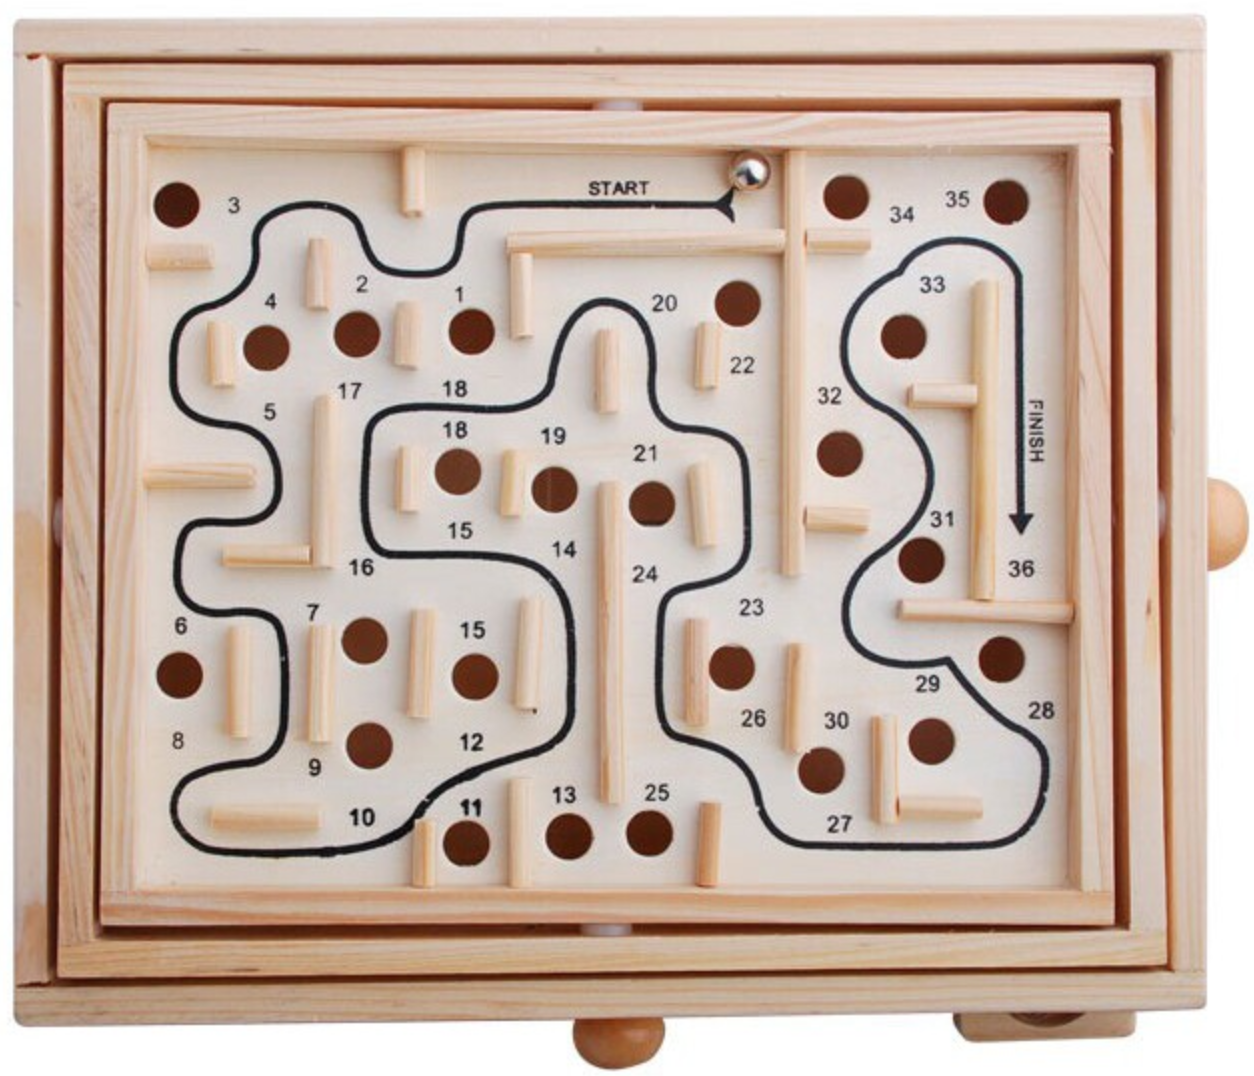
\includegraphics[width=0.65\textwidth]{images/wooden_game_board}
    \caption{The wooden game board, with the path to follow. Source:~\cite{wooden_board}}
    \label{fig:wooden_board}
\end{figure}

\subsection{Unity game board}\label{subsec:unity-game-board}
To closely approximate the movement and behavior of the marble in this physics based skill game,
Unity's built-in physics engine (PhysX3).
This system provides several components that can be attached to game objects, to ensure specific behaviors.
A game object in Unity defines the base for any entity in the given scene.
\begin{itemize}
    \item{Collider3D}: The Collider3D component can be added to any game object, either static or dynamic, to simulate the contact points of hard surfaces, like the marble or the game board.
    The shape is usually defined by or similar to the actual 3D model.
    This component can serve two purposes.
    It either behaves like a collider or, if specified by a flag, acts as a trigger, meaning it's not bouncing off other game objects.
    Instead it sends out a trigger signal.
    \item{Rigidbody3D}: To add game objects to the physics simulation that are affected by gravity, the Rigidbody3D component with the associated flag can be added to game objects with a Collider3D.
\end{itemize}
With these two simple components and a C\# script the controls and gameplay can be simulated.\\
In addition to the original game board, some modifications had to be made:
\begin{enumerate}
    \item{Top cover}: To make sure that the marble can't bounce out of the labyrinth, a transparent Collider3D has been
    added as a lid on top of the labyrinth.
    \item{Holes}: The board has holes in the base plate in the same positions as the original game board.
    Another Collider3D, but as a trigger, has been added below the game board to know, when the marble has fallen through a hole.
    The game will reset, if this event occurs.
    \item{Checkpoints}: Since the rules state that the marble has to follow the given path a checkpoint system has been implemented to ensure that the agent learns the correct behavior.
    A marble can only pass through the current checkpoint in line, otherwise the game will reset.
\end{enumerate}